% Created 2022-07-06 Wed 08:59
% Intended LaTeX compiler: pdflatex
\documentclass[bigger]{beamer}
\usepackage[utf8]{inputenc}
\usepackage[T1]{fontenc}
\usepackage{graphicx}
\usepackage{grffile}
\usepackage{longtable}
\usepackage{wrapfig}
\usepackage{rotating}
\usepackage[normalem]{ulem}
\usepackage{amsmath}
\usepackage{textcomp}
\usepackage{amssymb}
\usepackage{capt-of}
\usepackage{hyperref}
\usetheme[progressbar=foot]{metropolis}
\author{Edmund Miller}
\date{2022-07-05 Wed}
\title{Viral Integration}
\hypersetup{
 pdfauthor={Edmund Miller},
 pdftitle={Viral Integration},
 pdfkeywords={},
 pdfsubject={},
 pdfcreator={Emacs 29.0.50 (Org mode 9.6)}, 
 pdflang={English}}
\usepackage{biblatex}
\addbibresource{~/sync/reference/bibliography.bib}
\addbibresource{~/sync/reference/biochemistry.bib}
\addbibresource{~/sync/reference/genomics.bib}
\addbibresource{~/sync/reference/molecular_biology.bib}
\addbibresource{~/sync/reference/molecular_biology_project.bib}
\addbibresource{~/sync/reference/books.bib}
\begin{document}

\maketitle

\section*{nf-core/viralintegration}
\label{sec:org4d4fbbc}

\begin{frame}[label={sec:orgb1869e7},fragile]{Background}
 \begin{itemize}
\item Started out wondering if we could look for Viral Integration in 1000 Genomes, inspired by \href{http://oncodb.org/}{OncoDB}
\item Original: \texttt{bam2fastq} unaligned reads => nf-core/sarek (WGS) with a custom
reference
\item Met Robert Allaway, Principal Scientist @ Sage Bionetwork on nf-core
\end{itemize}
\end{frame}

\begin{frame}[label={sec:org69ce5b1}]{Background}
\begin{center}
\includegraphics[width=.9\linewidth]{/home/emiller/.config/emacs/.local/cache/org-persist/a6/1bb1de-29cf-406b-84e3-a27f8fa75cc2-8346acd07f56aae3cc7f70f26a008bff.png}
\end{center}
\end{frame}

\begin{frame}[label={sec:orgf4c511d}]{Approaches}
\begin{itemize}
\item MetaPhlAn (Robert)
\item CTAT - Virus Integration Finder (ctat-VIF) (Alyssa Briggs)
\item BLASTBox (Edmund)
\end{itemize}
\end{frame}

\begin{frame}[label={sec:orgad28565}]{Why are we interested in Viral Integration?}
\begin{itemize}
\item Besides aberrant DNA methylation or RNA expression, another major cause of
cancer is viral infection (Oncoviruses)
\item Identification of oncovirus-related gene expression changes helps better
understand the mechanisms underlying virus-induced cancers
\item Lack of current research in the area utilizing new data
\end{itemize}
\end{frame}

\section*{CTAT - Virus Integration Finder}
\label{sec:orgb5655c7}

\begin{frame}[label={sec:org9c0c05c}]{CTAT - Virus Integration Finder}
\begin{itemize}
\item Capture evidence of virus-matching reads (consistent with an infection)
\item Identify and quantify evidence for viral insertion sites in the human genome
\item Provide interactive visualizations for evidence of virus-mapped reads and
virus insertion sites
\end{itemize}
\end{frame}

\begin{frame}[label={sec:org38192b4}]{CTAT - Virus Integration Finder}
\begin{itemize}
\item Trinity Cancer Transcriptome Analysis Toolkit - CWL
\item Takes DNA-seq or RNA-seq
\item Requires a CTAT genome lib supplemented with viral genomes (They provide a virusdb fasta).
\end{itemize}
\end{frame}

\begin{frame}[label={sec:org04235c6}]{CTAT - DAG}
\begin{center}
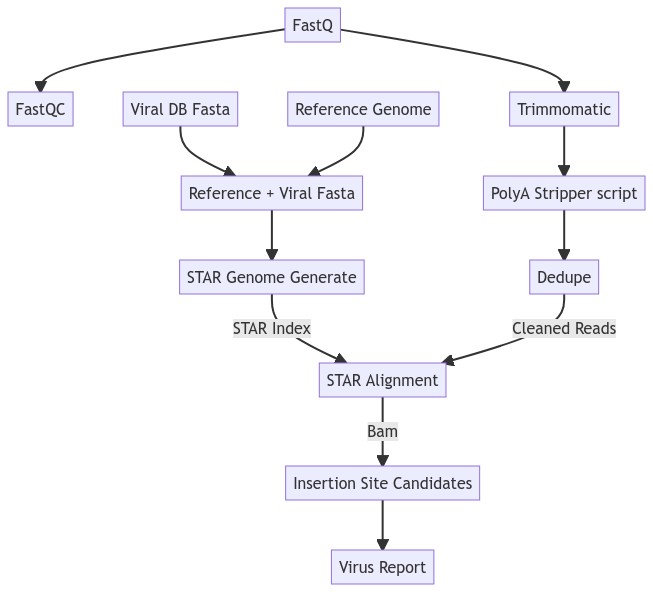
\includegraphics[height=0.20\linewidth]{/home/emiller/src/personal/edmundmiller-dev/static/org-attach/de/1b3c29-d7ca-4e44-8708-c72053d52682/_20220706_081414screenshot.png}
\end{center}
\end{frame}


\begin{frame}[label={sec:orgd810fd9}]{CTAT - Virus Integration Finder}
\footnotesize
\begin{center}
\begin{tabular}{lrllrllrrrr}
chrA & coordA & orientA & chrB & coordB & orientB & prelim.primary\textsubscript{brkpt}\textsubscript{type} & prelim.total & split & span & total\\
\hline
chr11 & 117344940 & + & HPV16 & 1215 & + & Split & 117 & 33 & 79 & 112\\
chr18 & 73320805 & + & HPV16 & 7409 & - & Split & 168 & 31 & 72 & 103\\
chr6 & 64935774 & + & HPV16 & 4034 & - & Split & 177 & 30 & 70 & 100\\
HPV16 & 4029 & + & chr3 & 937922 & + & Split & 1 & 0 & 0 & 0\\
HPV16 & 1215 & - & chr11 & 108577428 & + & Split & 1 & 0 & 0 & 0\\
chr2 & 32018732 & + & HPV16 & 1215 & + & Split & 1 & 0 & 0 & 0\\
chr1 & 218562612 & + & HPV16 & 1215 & + & Split & 1 & 0 & 0 & 0\\
\end{tabular}
\end{center}
\end{frame}


\begin{frame}[label={sec:org458dba5}]{CTAT - Insertion Site Candidates}
\begin{center}
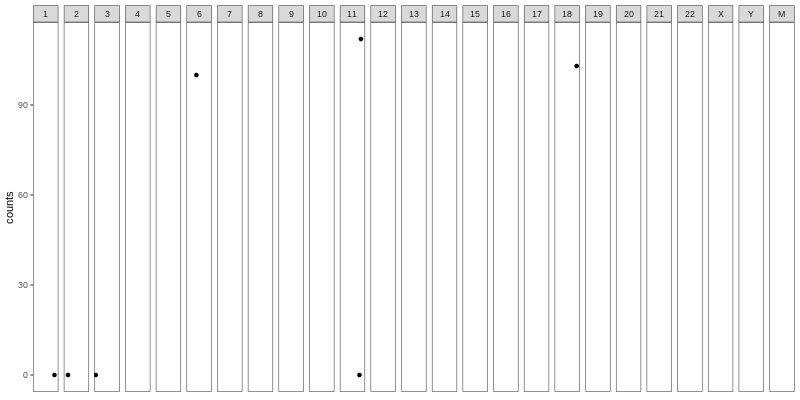
\includegraphics[width=.9\linewidth]{/home/emiller/src/personal/edmundmiller-dev/static/org-attach/0f/a01f6e-0bdc-49a0-8083-8e10c011cdb9/_20220705_222615screenshot.png}
\end{center}
\end{frame}


\begin{frame}[label={sec:org76567ff}]{CTAT - Virus Insertion Viewer}
\begin{center}
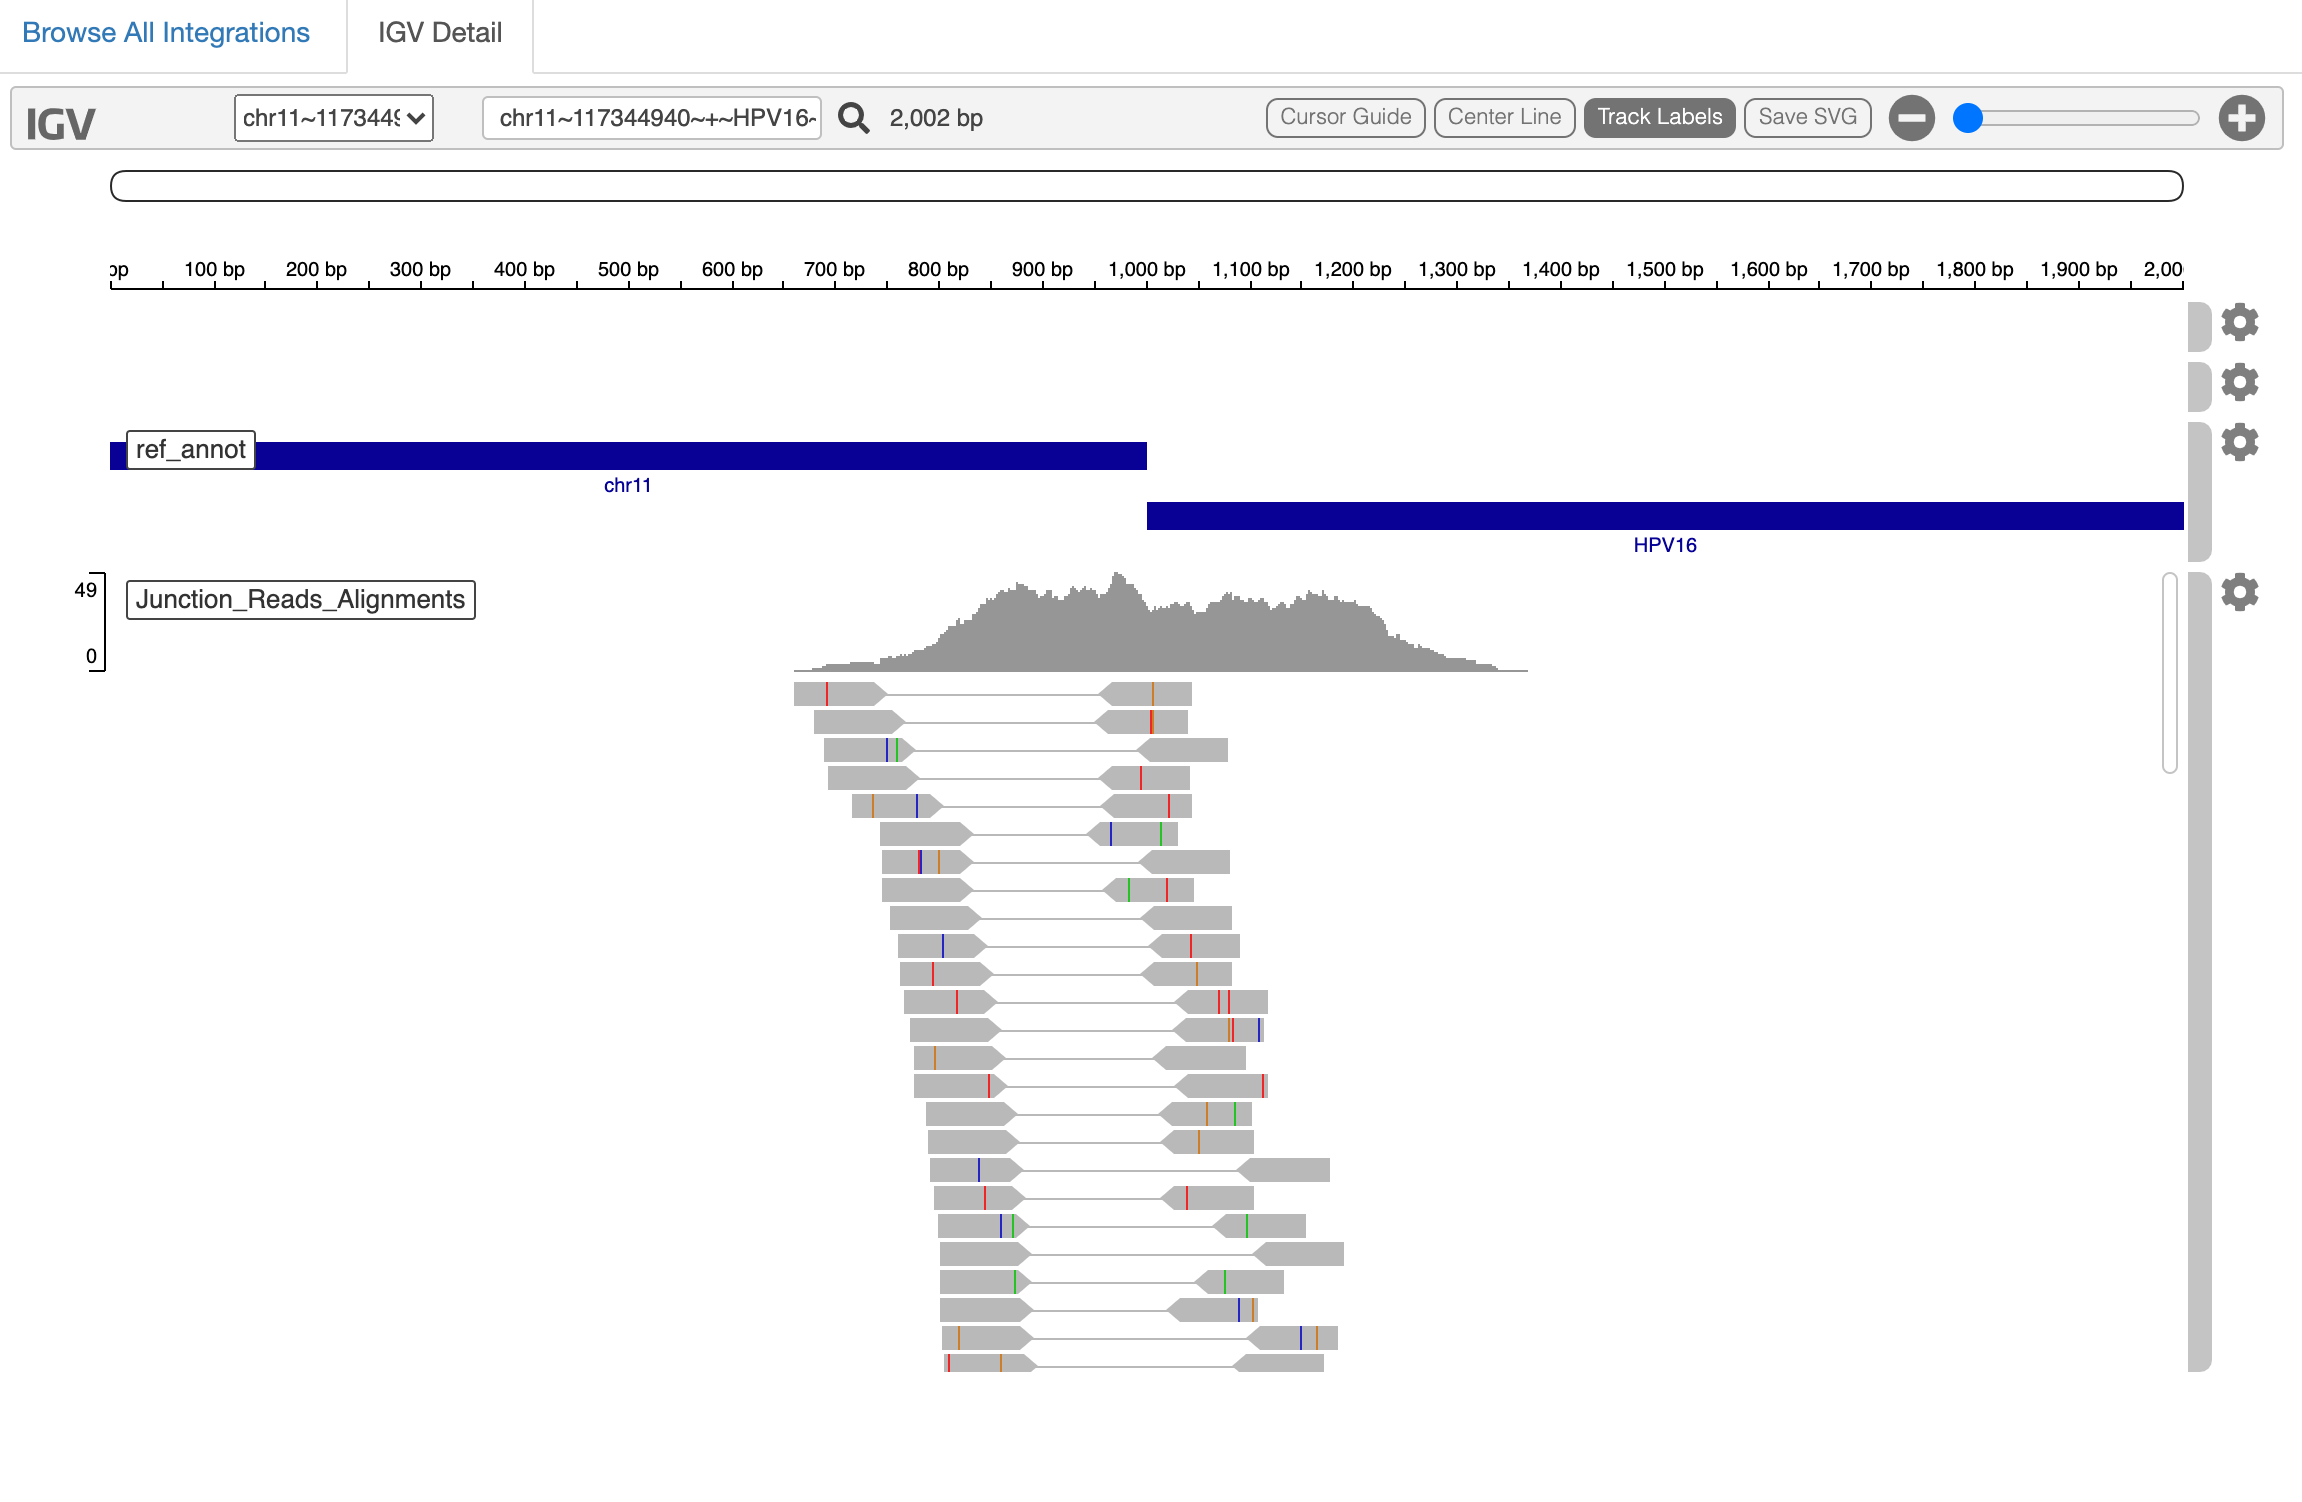
\includegraphics[height=0.4\linewidth]{/home/emiller/src/personal/edmundmiller-dev/static/org-attach/66/211082-d11c-4fd4-bbbd-00d997ec7f4d/_20220705_223158screenshot.png}
\end{center}
\end{frame}

\begin{frame}[label={sec:org0fb62ef}]{CTAT - Virus Infection Evidence Viewer}
\begin{itemize}
\item There may not be strong evidence for virus insertions
\item Detects reads aligning to the target virus sequence
\end{itemize}
\end{frame}

\begin{frame}[label={sec:org7e319a3}]{CTAT - Virus Infection Evidence Viewer}
\begin{center}
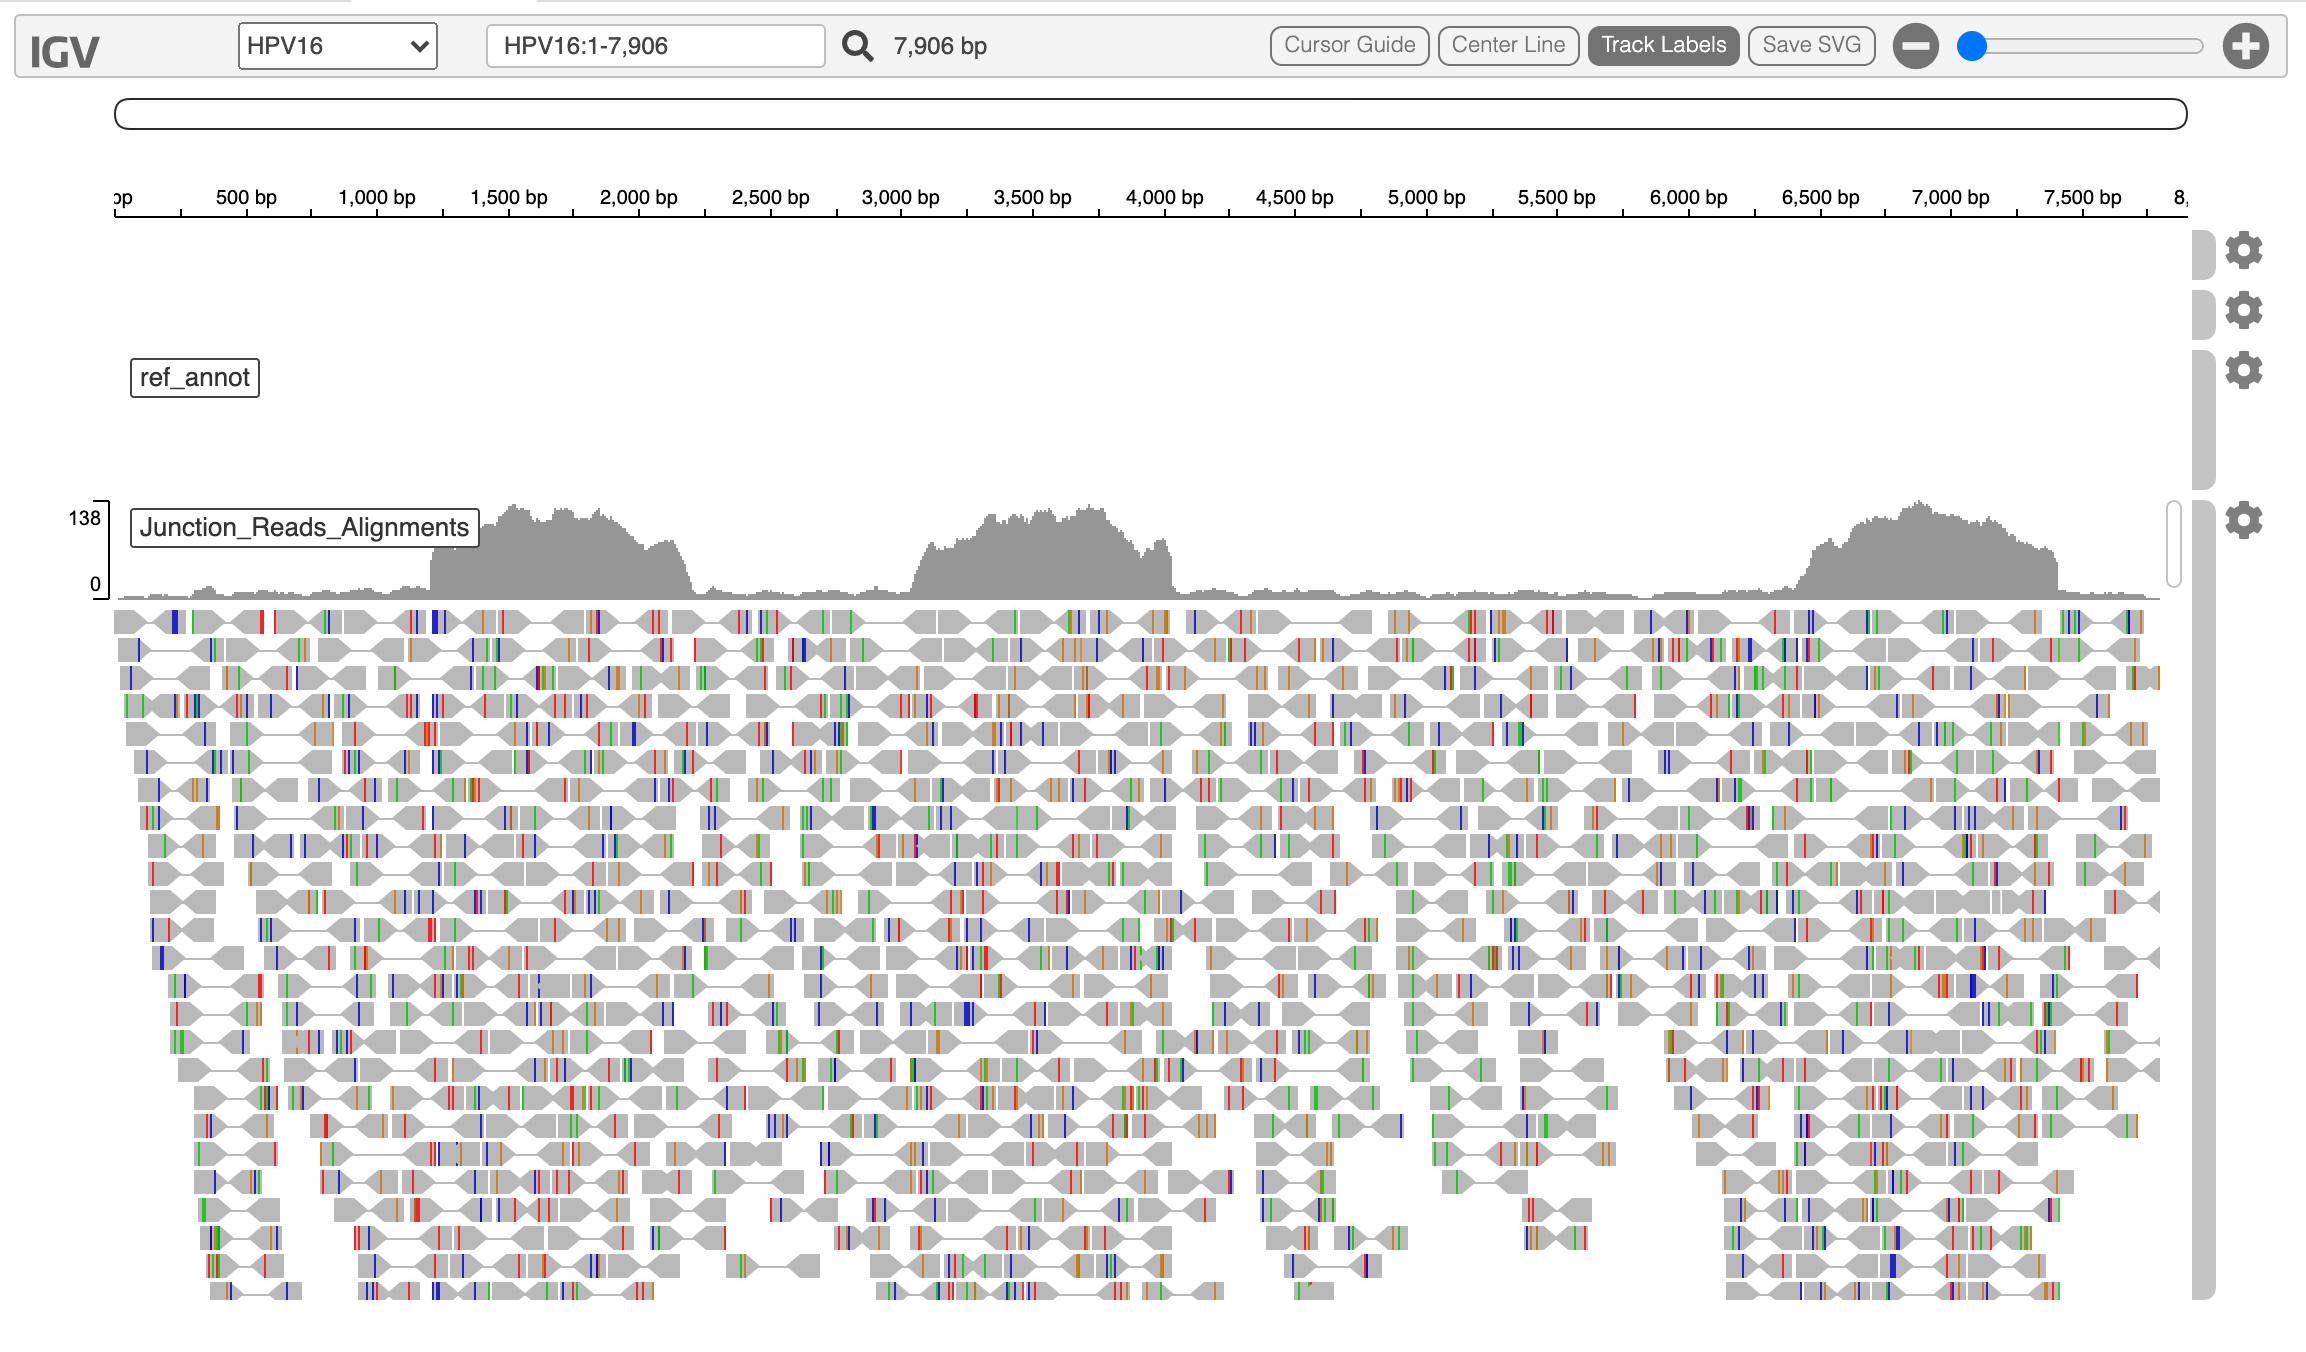
\includegraphics[height=0.25\linewidth]{/home/emiller/src/personal/edmundmiller-dev/static/org-attach/85/fec50f-b0cf-4721-98d0-3b1e5e56ba79/_20220706_085548screenshot.png}
\end{center}
\end{frame}


\section*{BLASTBox}
\label{sec:org7cfcf46}

\begin{frame}[label={sec:orgd0c6e09}]{BLASTBox}
\begin{itemize}
\item Main goal was to \alert{avoid realigning} thousands of high-coverage samples, by
pulling out unaligned reads
\item Found a similar study of TCGA data
\end{itemize}
\end{frame}

\begin{frame}[label={sec:org12c077d}]{BLASTBox - DAG}
\begin{center}
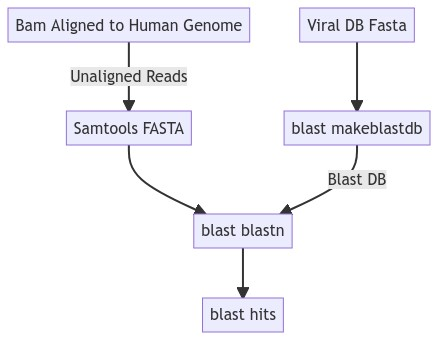
\includegraphics[width=.9\linewidth]{/home/emiller/src/personal/edmundmiller-dev/static/org-attach/8a/152476-d37a-4dcf-a5ba-c698b37bf2d6/_20220706_082010screenshot.png}
\end{center}
\end{frame}

\begin{frame}[label={sec:orgd29fa71}]{BLASTBox}
\begin{center}

\includegraphics[width=.9\linewidth]{/home/emiller/src/personal/edmundmiller-dev/static/org-attach/8d/1efa65-35ae-4394-95f6-a36ddd602529/_20220706_072610screenshot.png}
\end{center}
\end{frame}

\begin{frame}[label={sec:org6e1bdd1}]{Viral expression associated with GIA Highlights (2013)}
\begin{itemize}
\item Goal: Determine whether the presence of a virus is significantly associated
with tumors
\item 59\% of screened gastrointestinal adenocarcinomas (GIA) were positive for at
least one virus
\item Used a similar approach, BAM => BLAST
\end{itemize}
\end{frame}

\begin{frame}[label={sec:org2a13ece}]{BLASTBox Targets}
\begin{itemize}
\item 1000 Genomes 30x WGS
\item TCGA WGS
\item dbGaP
\end{itemize}
\end{frame}

\begin{frame}[label={sec:org69a800a}]{Initial Questions to ask}
\begin{itemize}
\item What parts of the sequence got integrated?
\item What parts of the sequence got tossed out?
\item Which one is potentially toxic/oncogenic
\end{itemize}
\end{frame}
\end{document}
